\documentclass{article}
\usepackage[utf8]{inputenc}
\usepackage{polski}
\usepackage{geometry}
\usepackage{pdfpages}
\usepackage{pdfpages}
\usepackage{listings}
\usepackage{listingsutf8}
\usepackage{multirow}
\usepackage{siunitx}
\usepackage{multirow}
\usepackage{booktabs}
\usepackage{tabularx}
\usepackage{placeins}
\usepackage{pdflscape}
\usepackage{colortbl}
\usepackage{listings}
\usepackage{listingsutf8}

\geometry{
a4paper,
total={170mm,257mm},
left=20mm,
top=20mm
}
\newcolumntype{Y}{>{\centering\arraybackslash}X}
% \renewcommand\thesection{}
\lstset{%
literate=%
 {ą}{{\k{a}}}1
 {ę}{{\k{e}}}1
 {Ą}{{\k{A}}}1
 {Ę}{{\k{E}}}1
 {ś}{{\'{s}}}1
 {Ś}{{\'{S}}}1
 {ź}{{\'{z}}}1
 {Ź}{{\'{Z}}}1
 {ń}{{\'{n}}}1
 {Ń}{{\'{N}}}1
 {ć}{{\'{c}}}1
 {Ć}{{\'{C}}}1
 {ó}{{\'{o}}}1
 {Ó}{{\'{O}}}1
 {ż}{{\.{z}}}1
 {Ż}{{\.{Z}}}1
 {ł}{{\l{}}}1
 {Ł}{{\l{}}}1
}

\title{Technika Cyfrowa\\
Sprawozdanie - FPGA}
\author{Maciej Trątnowiecki}
\date{AGH, Semestr Letni, 2020}

\begin{document}
\lstset{ 
  backgroundcolor=\color{white},   % choose the background color; you must add \usepackage{color} or \usepackage{xcolor}; should come as last argument
  basicstyle=\footnotesize,        % the size of the fonts that are used for the code
  breakatwhitespace=false,         % sets if automatic breaks should only happen at whitespace
  breaklines=true,                 % sets automatic line breaking
  captionpos=b,                    % sets the caption-position to bottom
  commentstyle=\color{mygreen},    % comment style
  deletekeywords={...},            % if you want to delete keywords from the given language
  escapeinside={\%*}{*)},          % if you want to add LaTeX within your code
  %extendedchars=true,              % lets you use non-ASCII characters; for 8-bits encodings only, does not work with UTF-8
  firstnumber=1000,                % start line enumeration with line 1000
  frame=single,	                   % adds a frame around the code
  keepspaces=true,                 % keeps spaces in text, useful for keeping indentation of code (possibly needs columns=flexible)
  keywordstyle=\color{blue},       % keyword style
  language=Octave,                 % the language of the code
  morekeywords={*,...},            % if you want to add more keywords to the set
  numbers=left,                    % where to put the line-numbers; possible values are (none, left, right)
  numbersep=5pt,                   % how far the line-numbers are from the code
  numberstyle=\tiny\color{mygray}, % the style that is used for the line-numbers
  rulecolor=\color{black},         % if not set, the frame-color may be changed on line-breaks within not-black text (e.g. comments (green here))
  showspaces=false,                % show spaces everywhere adding particular underscores; it overrides 'showstringspaces'
  showstringspaces=false,          % underline spaces within strings only
  showtabs=false,                  % show tabs within strings adding particular underscores
  stepnumber=2,                    % the step between two line-numbers. If it's 1, each line will be numbered
  stringstyle=\color{mymauve},     % string literal style
  tabsize=2,	                   % sets default tabsize to 2 spaces
  title=\lstname                   % show the filename of files included with \lstinputlisting; also try caption instead of title
}
    \maketitle
    \section{Opis zrealizowanego projektu}
        W ramach zadania praktycznego przygotowałem implementację algorytmu wyświetlającego na dwóch wyświetlaczach siedmiosegmentowych animację węża. Algorytm zaimplementowałem w dwóch wersjach - w języku SystemVerilog i VHDL dla płytki rozwojowej Altera UP2 wyposażonej w układ FPGA FLEX 10KE EPF10K70RC240-4. Wykorzystałem środowisko Quartus II 9.0SP2, w którym przeprowadziłem symulację działania programu. \\
        
        
        \begin{center}
            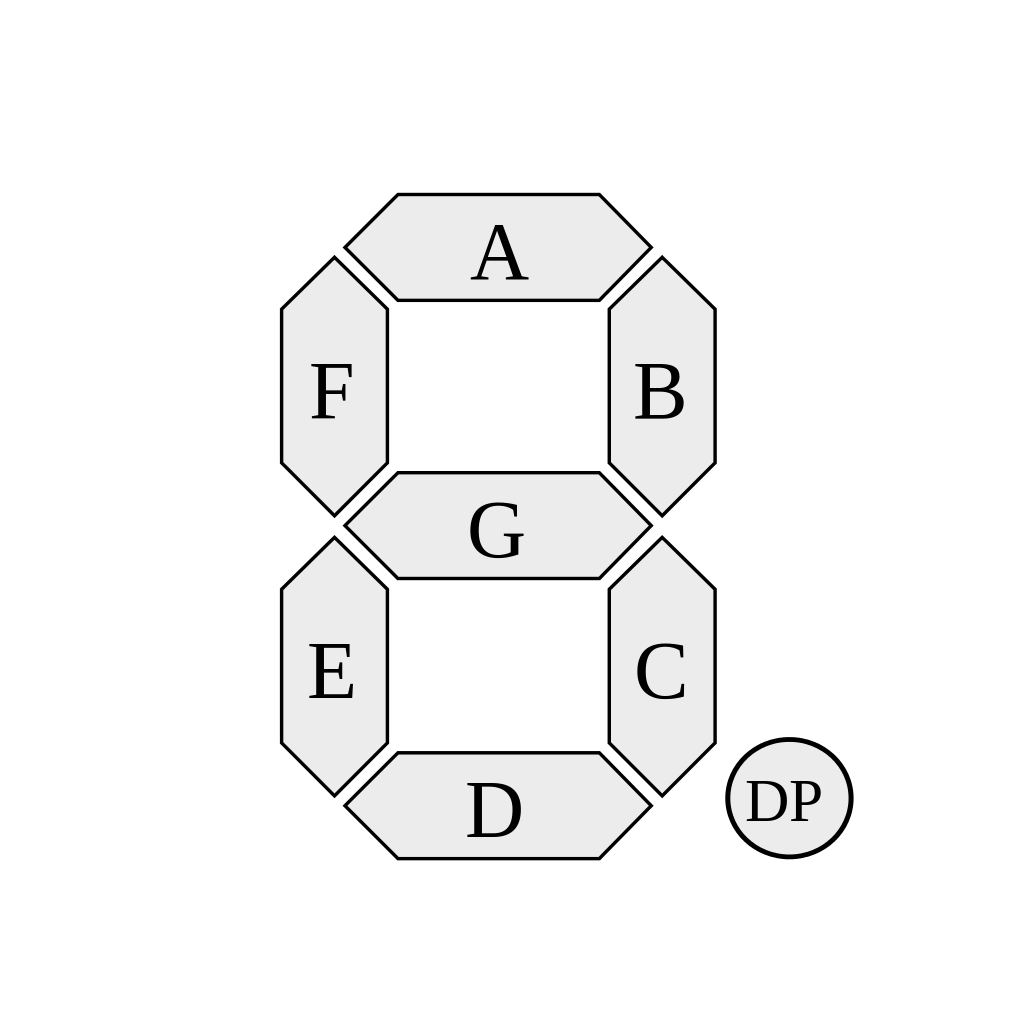
\includegraphics[height=5cm]{reports/img/7seg.png}\\
        \end{center}

    
    
    \section{Implementacja w języku SystemVerilog}
        \lstinputlisting[language=SystemVerilog]{../simulations/FPGA/snake_verilog/snake.sv}
    
    \section{Implementacja w języku VHDL}
        \lstinputlisting[language=VHDL]{../simulations/FPGA/snake_vhdl/snake.vhd}
    
    \section{Przydział pinów}
    
    \section{Symulacja działania programu}
    
    
\end{document}
